\thispagestyle{fancy}

\begin{appendices}

\chapter{Derivations}
\label{ax:derivations}

\section*{Investment Optimization in Tullock Contest}

A player $i$ wants to find the $I^*$ that maximizes his or her expected profit as expressed in the maximization problem:


\begin{equation}
    \underset{I_i}{\text{max}}\quad\mathbb{E}\Pi_i(I_i,I_j) = \frac{I_i}{I_i + \sum_{j\neq i}^n I_{j}}\mathbb{V} - I_i
\label{eq:exp_util_anex}
\end{equation}

Where $n$ is the  number of participants in the game.\\
Let us assume that the valuation of the game $\mathbb{V}$ is equal for all players and hence, that the optimal investment $I^{*}$ is equal for everyone. At the maximum of function \ref{eq:exp_util_anex} holds:
\begin{flalign*}
    \frac{d}{dI_i}(\frac{I_i\mathbb{V}}{I_i + \sum_{j\neq i}^n I_{j}} - I_i) = 0 &&
\end{flalign*}
which after deriving using the quotient rule results in:
\begin{flalign*}
    \frac{\mathbb{V}(I_i + \sum_{j\neq i}^n I_{j})-I_i\mathbb{V}}{(I_i + \sum_{j\neq i}^n I_{j})^2}-1&&
\end{flalign*}
Since we know that at the maximum $I_i^{*}=I_{-i}^{*}=I^{*}$ holds, we can simplify:
\begin{flalign*}
    \frac{n\mathbb{V}I^*-\mathbb{V}I^*}{(nI^*)^2}-1 = 0&&
\end{flalign*}
We further simplify to:
\begin{flalign*}
    \frac{\mathbb{V}\bcancel{I^*}(n-1)}{n^2I^{\bcancel{*2}}} = 1&&
\end{flalign*}
Which gives equation \ref{eq:opt_last}:
\begin{flalign*}
    I^{*} = \frac{n-1}{n^2}\mathbb{V}
\end{flalign*}

\chapter{Tables}

\begin{table}[!htbp] \centering
\begin{tabular}{@{\extracolsep{5pt}}lcc} 
\multicolumn{3}{l}{Wilcoxon rank sum test with continuity correction}\\
\\[-1.8ex]\hline 
\hline \\[-1.8ex] 
\multicolumn{1}{l}{Piece Rate} & \multicolumn{1}{c}{Statistic} & \multicolumn{1}{c}{p-value}\\
\hline \\[-1.8ex]
High & 1186.5 & 0.8006\\
Low & 1070 & 0.5462\\
\hline \\[-1.8ex] 
\hline \\[-1.8ex]
\multicolumn{3}{l}{\footnotesize{Null Hypothesis: Difference in production between treatments is equal to 0}}\\[2ex]
\end{tabular}
  \caption{Comparison of productions in the benchmarking rounds between treated and non treated groups} 
  \label{tab:bench_prods_test} 
\end{table} 


    \begin{figure}
        \centering
        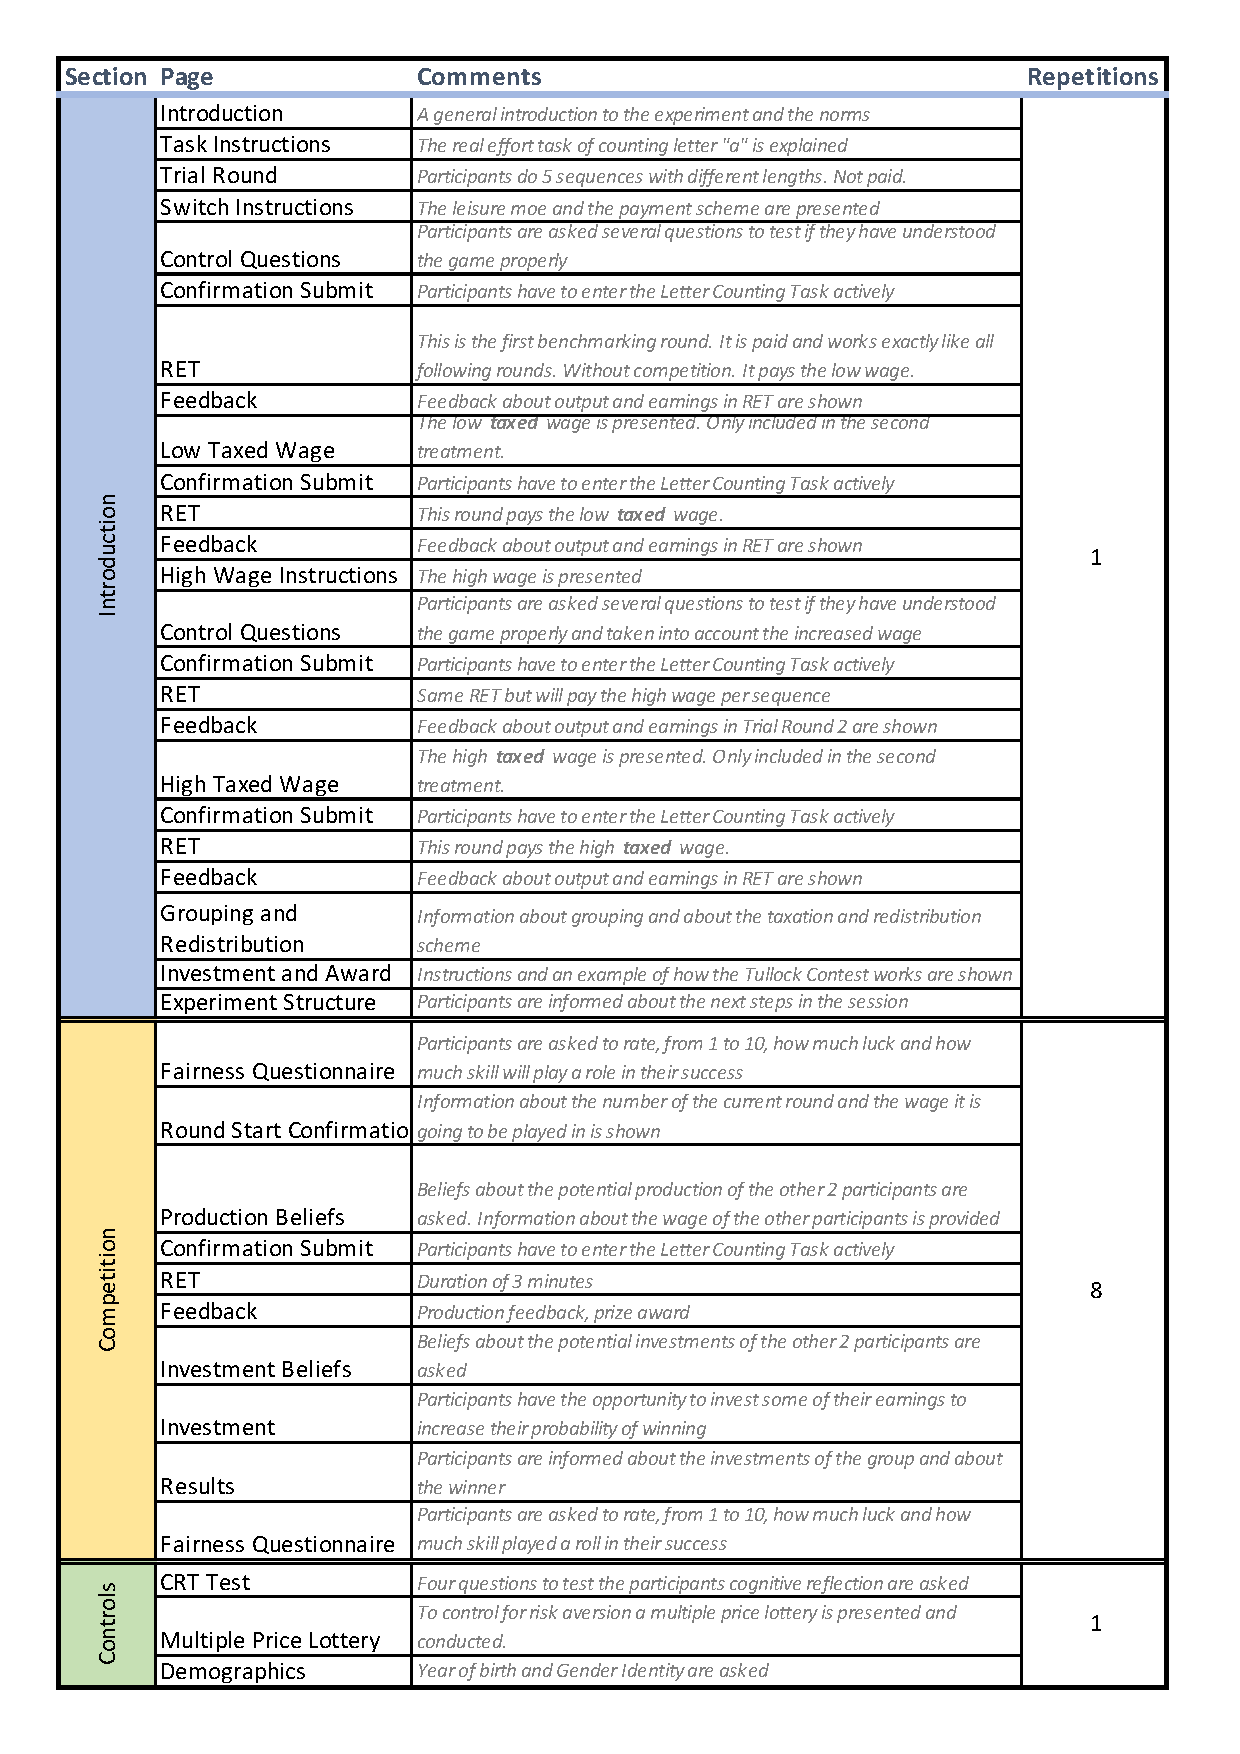
\includegraphics[width=\textwidth]{graphs/Experimental_Design.pdf}
        \caption{Detailed structure of the experiment}
        \label{tab:exp_design}
    \end{figure}
    
\begin{table}[!htbp] \centering 
  \caption{GLMM Probability of Winning} 
  \label{ax:glm_prob} 
\begin{tabular}{@{\extracolsep{5pt}}lc} 
\\[-1.8ex]\hline 
\hline \\[-1.8ex] 
\\[-1.8ex] & \multicolumn{1}{c}{Probability of Winning} \\ 
\\[-1.8ex] & (3)\\ 
\hline \\[-1.8ex] 
 treatment & $-$0.091 \\ 
  & (0.218) \\ 
  &  \\ 
 available income & 0.044$^{***}$  \\ 
  & (0.008) \\ 
  & \\ 
 was winner & $-$0.056 \\ 
  & (0.121) \\ 
  & \\ 
 gender (male) & 0.317\\ 
   & (0.225) \\ 
   & \\ 
 CRT Score  & $-$0.036 \\ 
  & (0.113) \\ 
  & \\ 
 risk aversion & 0.036 \\ 
  & (0.049) \\ 
  & \\ 
 valuation & 0.060 \\ 
  & (0.038) \\ 
  & \\ 
 mean investment belief & 0.002 \\ 
  & (0.009) \\ 
  & \\
 cumulative wins & $-$0.037 \\ 
  & (0.028) \\ 
  & \\ 
 Constant & $-$2.364$^{***}$ \\ 
  & (0.650) \\ 
  & \\ 
  \hline
Observations & 672 \\ 
Log Likelihood & 3801.8 \\ 
Akaike Inf. Crit. & $-$7575.6 \\ 
Bayesian Inf. Crit. & $-$7512.5 \\
\hline
Num. groups: participant:group     &   96   \\
Num. groups: group               &    32  \\
Num. groups: round               & 7        \\
\hline
Var: participant:group (Intercept) &  0.872     \\
Var: group (Intercept) &          0.00     \\
Var: round (Intercept)  &          0.00    \\
\hline
\hline \\[-1.8ex] 
\textit{Notes:} & \multicolumn{1}{l}{$^{***}$Significant at the 1 percent level.} \\ 
 & \multicolumn{1}{l}{$^{**}$Significant at the 5 percent level.} \\ 
 & \multicolumn{1}{l}{$^{*}$Significant at the 10 percent level.} \\ 
\end{tabular} 
\end{table} 

\end{appendices}